%\begin{figure}[h]
%\hspace*{\fill}
%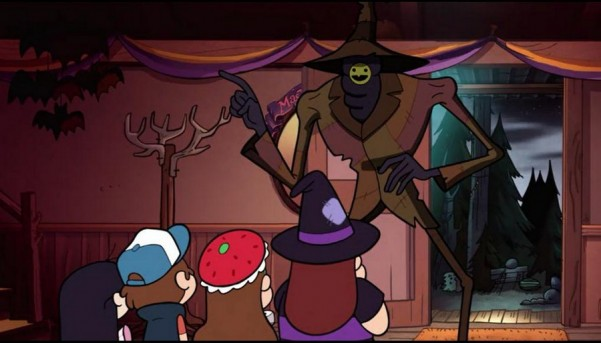
\includegraphics[width=\linewidth,natwidth=601,natheight=343]{H.jpg}
%\hspace*{\fill}
%\end{figure}


Во время Хеллоуина Гравити Фолз наводнили конфетные монстры. Диппер, Мейбл и их друзья не хотят портить себе праздник, ведь они ждали его целый год, поэтому они пытаются собрать побольше сладостей и победить монстров, одновременно. Чтобы прогнать монстра необходимо отдать ему некоторое количество конфет. В результате весь вечер ребята бегали от дома к дому, собирая сладкое у старушек и отстреливаясь от чудищ конфетами. В конце вечера у них оказалось $n$ конфет. Диппер помнит, на сколько менялось количество конфет, но он совершенно забыл, как именно оно менялось каждый раз. Помогите Дипперу определить, как изменялось количество сладостей каждый раз, если в начале вечера у них не было ни одной конфеты.

\InputFile
В первой строке находятся числа $N (2 \le N \le 12)$ и $S(-1000000 \le S \le 1000000)$, означающие количество изменений и текущее количество конфет, соотвественно. В следующей строке N чисел через пробел~---~величину каждого изменения $(0 \le X_i \le 50000)$

\OutputFile
Если получить требуемый результат невозможно, вывести \t{No solution}. Если можно, то вывести равенство. Если решение не единственное, вывести любое. Числа и знаки нужно выводить через пробел.

\SAMPLES

